\documentclass[tikz,border=8pt]{standalone}
% Shared look for every TikZ diagram. Load with \input{../../tools/tikz-style.tex}
\usepackage[T1]{fontenc}
\usepackage{lmodern}
\renewcommand{\sfdefault}{lmr}  % diagrams use the same serif as the text
\usetikzlibrary{arrows.meta, positioning, shapes.geometric, calc, fit, backgrounds}
\definecolor{cblue}{HTML}{4C78A8}
\definecolor{corange}{HTML}{F58518}
\definecolor{cgreen}{HTML}{54A24B}
\definecolor{cred}{HTML}{E45756}
\definecolor{cpurple}{HTML}{B279A2}
\definecolor{cgrey}{HTML}{6B6B6B}
\tikzset{
  every picture/.style={font=\sffamily, line width=1.2pt},
  box/.style={draw=#1, fill=#1!12, rounded corners=4pt, align=center, inner sep=7pt, minimum height=1.1cm},
  box/.default=cgrey,
  arrow/.style={-{Stealth[length=3mm]}, draw=cgrey, line width=1.4pt},
  title/.style={font=\sffamily\bfseries\Large},
  note/.style={font=\sffamily\small, text=cgrey, align=center},
}
\AtBeginDocument{\hyphenpenalty=10000 \exhyphenpenalty=10000}

\usepackage{amssymb}
% #1 panel name, #2 x offset, #3 y offset: a box with faces 1..6 as nodes #1-1 ... #1-6
\newcommand{\faces}[3]{%
  \draw[thick, rounded corners, draw=cgrey] (#2,#3) rectangle ++(6.4,2.0);
  \foreach \n in {1,...,6} \node[font=\sffamily\Large, inner sep=2pt] (#1-\n) at ({#2-0.02+\n*0.92},{#3+1.0}) {\n};}
\tikzset{ev/.style={draw=#1, fill=#1!20, rounded corners=10pt, inner sep=4pt, thick}}
\begin{document}
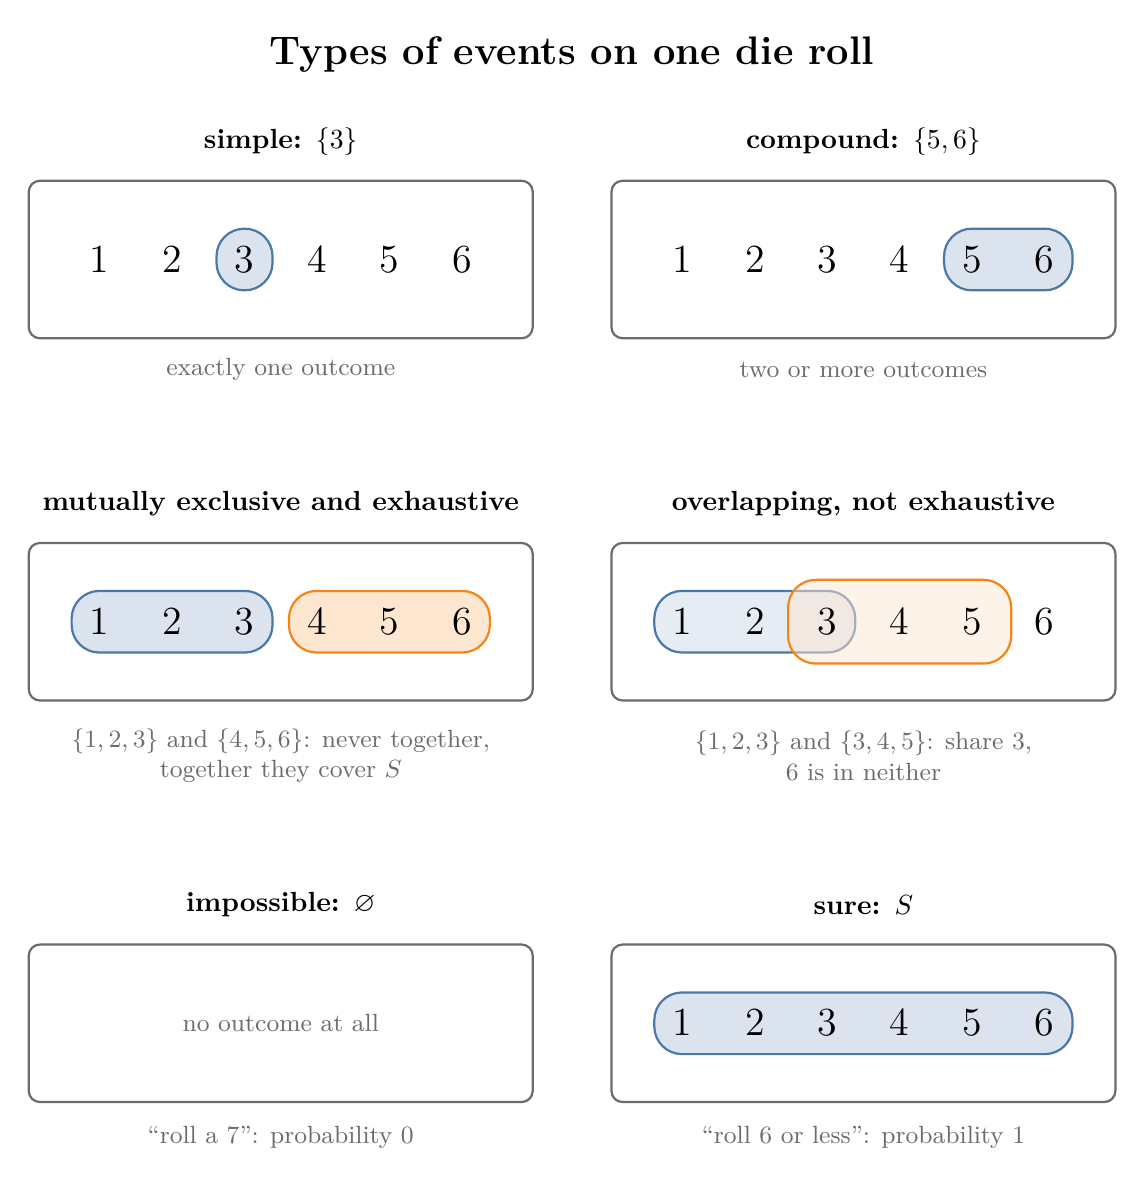
\begin{tikzpicture}[x=1cm, y=1cm]
  \node[title] at (6.9,11.0) {Types of events on one die roll};
  % row 1
  \node[font=\sffamily\bfseries] at (3.2,9.9) {simple: $\{3\}$};
  \faces{a}{0}{7.4}
  \node[note] at (3.2,7.0) {exactly one outcome};
  \node[font=\sffamily\bfseries] at (10.6,9.9) {compound: $\{5, 6\}$};
  \faces{b}{7.4}{7.4}
  \node[note] at (10.6,7.0) {two or more outcomes};
  % row 2
  \node[font=\sffamily\bfseries] at (3.2,5.3) {mutually exclusive and exhaustive};
  \faces{c}{0}{2.8}
  \node[note, align=center] at (3.2,2.1) {$\{1,2,3\}$ and $\{4,5,6\}$: never together,\\ together they cover $S$};
  \node[font=\sffamily\bfseries] at (10.6,5.3) {overlapping, not exhaustive};
  \faces{d}{7.4}{2.8}
  \node[note, align=center] at (10.6,2.1) {$\{1,2,3\}$ and $\{3,4,5\}$: share 3,\\ 6 is in neither};
  % row 3
  \node[font=\sffamily\bfseries] at (3.2,0.2) {impossible: $\varnothing$};
  \draw[thick, rounded corners, draw=cgrey] (0,-2.3) rectangle ++(6.4,2.0);
  \node[note] at (3.2,-1.3) {no outcome at all};
  \node[note] at (3.2,-2.75) {``roll a 7'': probability 0};
  \node[font=\sffamily\bfseries] at (10.6,0.2) {sure: $S$};
  \faces{e}{7.4}{-2.3}
  \node[note] at (10.6,-2.75) {``roll 6 or less'': probability 1};
  \begin{scope}[on background layer]
    \node[ev=cblue, fit=(a-3)] {};
    \node[ev=cblue, fit=(b-5)(b-6)] {};
    \node[ev=cblue, fit=(c-1)(c-3)] {};
    \node[ev=corange, fit=(c-4)(c-6)] {};
    \node[ev=cblue, fit=(d-1)(d-3), fill opacity=0.7] {};
    \node[ev=corange, fit=(d-3)(d-5), inner sep=8pt, fill opacity=0.5] {};
    \node[ev=cblue, fit=(e-1)(e-6)] {};
  \end{scope}
\end{tikzpicture}
\end{document}
